\documentclass[14pt, a4paper]{article}

\usepackage[utf8]{inputenc}

\usepackage{graphicx}

\title{Python programming language.}
\author{Alexei Buzuma}


\begin{document}


	\maketitle
	
	\begin{center}
		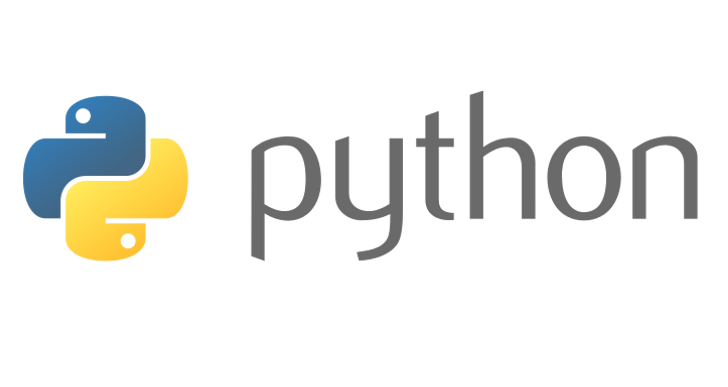
\includegraphics[width=0.7\textwidth]{n.png}
	\end{center}
	\newpage
	\begin{enumerate}
		\item Introduction:
		\begin{itemize}			
			\item What is Python.
			\item History of Python.
			\item Versions.
			\item Installation.
			\item Hello world!
			\item Python keywords.
			\item Indentation is very important!
			\item Quotes.
			\item Comments.
			\item Type of variables.
		\end{itemize}
		
		\item Work with objects:
		\begin{itemize}
			\item Assignment, deleting, conversion.
			\item Immutable vs Mutable
			\begin{itemize}
				\item list, dict, set, object
				\item tuple, int, float, string
			\end{itemize}
			
		\end{itemize}
		
		\item Operators:
		\begin{itemize}
			\item Arithmetic operators
			\item Comparison operators
			\item Assignment operators
			\item Bit operations
			\item Identity Operators(is, is not)
			\item Membership Operators(in, not in)
			\item Priority of operations
		\end{itemize}
		
		\item Conditionals:
		\begin{itemize}
			\item if... else...
			\item if... elif...
			\item one-line if
		\end{itemize}
		
		\item Cycles:
		\begin{itemize}
			\item for
			\item while
			\item else in cycles
			\item break, continue
		\end{itemize}
		
		\item Numbers:
		\begin{itemize}
			\item int, long, float, complex
			\item import math
			\item import random
		\end{itemize}
		
		\item Strings:
		\begin{itemize}
			\item .format and \%
			\item r'expression' and u'expression'
			\item methods
		\end{itemize}
		
		\item Slices
		
		\item Type system
		
		\item Iterators and Generators:
		\begin{itemize}
			\item list comprehensions
			\item dict comprehensions
			\item set comprehensions
			\item Iterators
		\end{itemize}
		
		\item Files and I/O
		
		\item Context managers
		
		\item Functions:
		\begin{itemize}
			\item Area of visibility
			\item lambda
			\item locals(); globals()
			\item function as object
		\end{itemize}
		
		\item Modules:
		\begin{itemize}
			\item import
			\item from ... import ...
			\item from ... import ... as ...
			\item Write your own module 
			\item dir()
			\item reload()
		\end{itemize}
		
		\item OOP:
		\begin{itemize}
			\item Classes and objects
			\item Atributes
			\item public and private
			\item Garbage Collection
			\item Inheritance
			\item issubclass, isinstance
		\end{itemize}
		
		\item Exceptions:
		
		\item Magic methods:
		
		\item Metaprogramming:
		\begin{itemize}
			\item Decorators
			\item Metaclasses
		\end{itemize}
		
		\item Concurrency
		
		\item Standard library
		
		\item Unit testing
		
		\item High Performance Python
		
	\end{enumerate}
\end{document}